\chapter{Demo Facility}\label{cha:demoFacility}
Physical creation of the demo facility that showcases the possibilities of the chosen wearable in the process of order picking in a warehouse. As the demo facility is not yet existing the implementation cannot be discussed and explained here, this chapter will therefore focus on the planned infrastructure, the existing design and what is planned for the demo facility in the future. 

There is also a major difference between the demo facility task that will be explained in this report and the task given in the logwear website. \citep{website:logwear} The task that will be executed here will be creating a demo facility in a physical \gls{sandbox} environment and the task explained in the work package on the logwear homepage is about implementing the improved process, using a wearable, at a pilot company and observing the results.

\section{Infrastructure}
The infrastructure of the demo facility is divided into multiple areas:
\begin{description}
	\item[Mock WMS] \hfill \\
		A mock \gls{wms} that allows to store different orders and edit them to have a more realistic demo. While not all functionality has to given, the data has to be persistent and easily resettable to allow showcasing a demo case multiple times. The mock \gls{wms} is living on an azure server and is a \gls{mssql} database.
	\item[Rest API] \hfill \\
		A \gls{rest} \gls{api} that is used to connect to the mock \gls{wms} from an outside perspective, in this case from the communication layer, see subsection \ref{subsec:communication}.
	\item[Communication Layer] \hfill \\
		The communication layer will be living on a server with a connection to the \gls{db} \gls{api} and a connection to the wearable.
	\item[Wearable] \hfill \\
		The wearable will need to connect to the communication layer and process input and output.
\end{description}

The mock \gls{wms} and the \gls{rest} \gls{api} are insignificant parts of the implementation, therefore not a lot of thought was put into the decision on choosing these technologies was done out of curiosity for these technologies or being the most comfortable with them respectively.

\section{Demo Scenario}\label{sec:demoScenario}
The demo scenario explains the process that will be executed during the demo facility. Therefore describing the actions taken in detail, but ignoring how they will be executed, e.g. with or without a wearable. The original process can be seen in the appendix, figure \ref{fig:orderPickingProcessDiagram}. For the actual scenario for the demo facility an activity diagram was created, that can be seen in figure \ref{fig:activityDemoScenario}. 

\begin{figure}[htbp]
	\begin{center}
	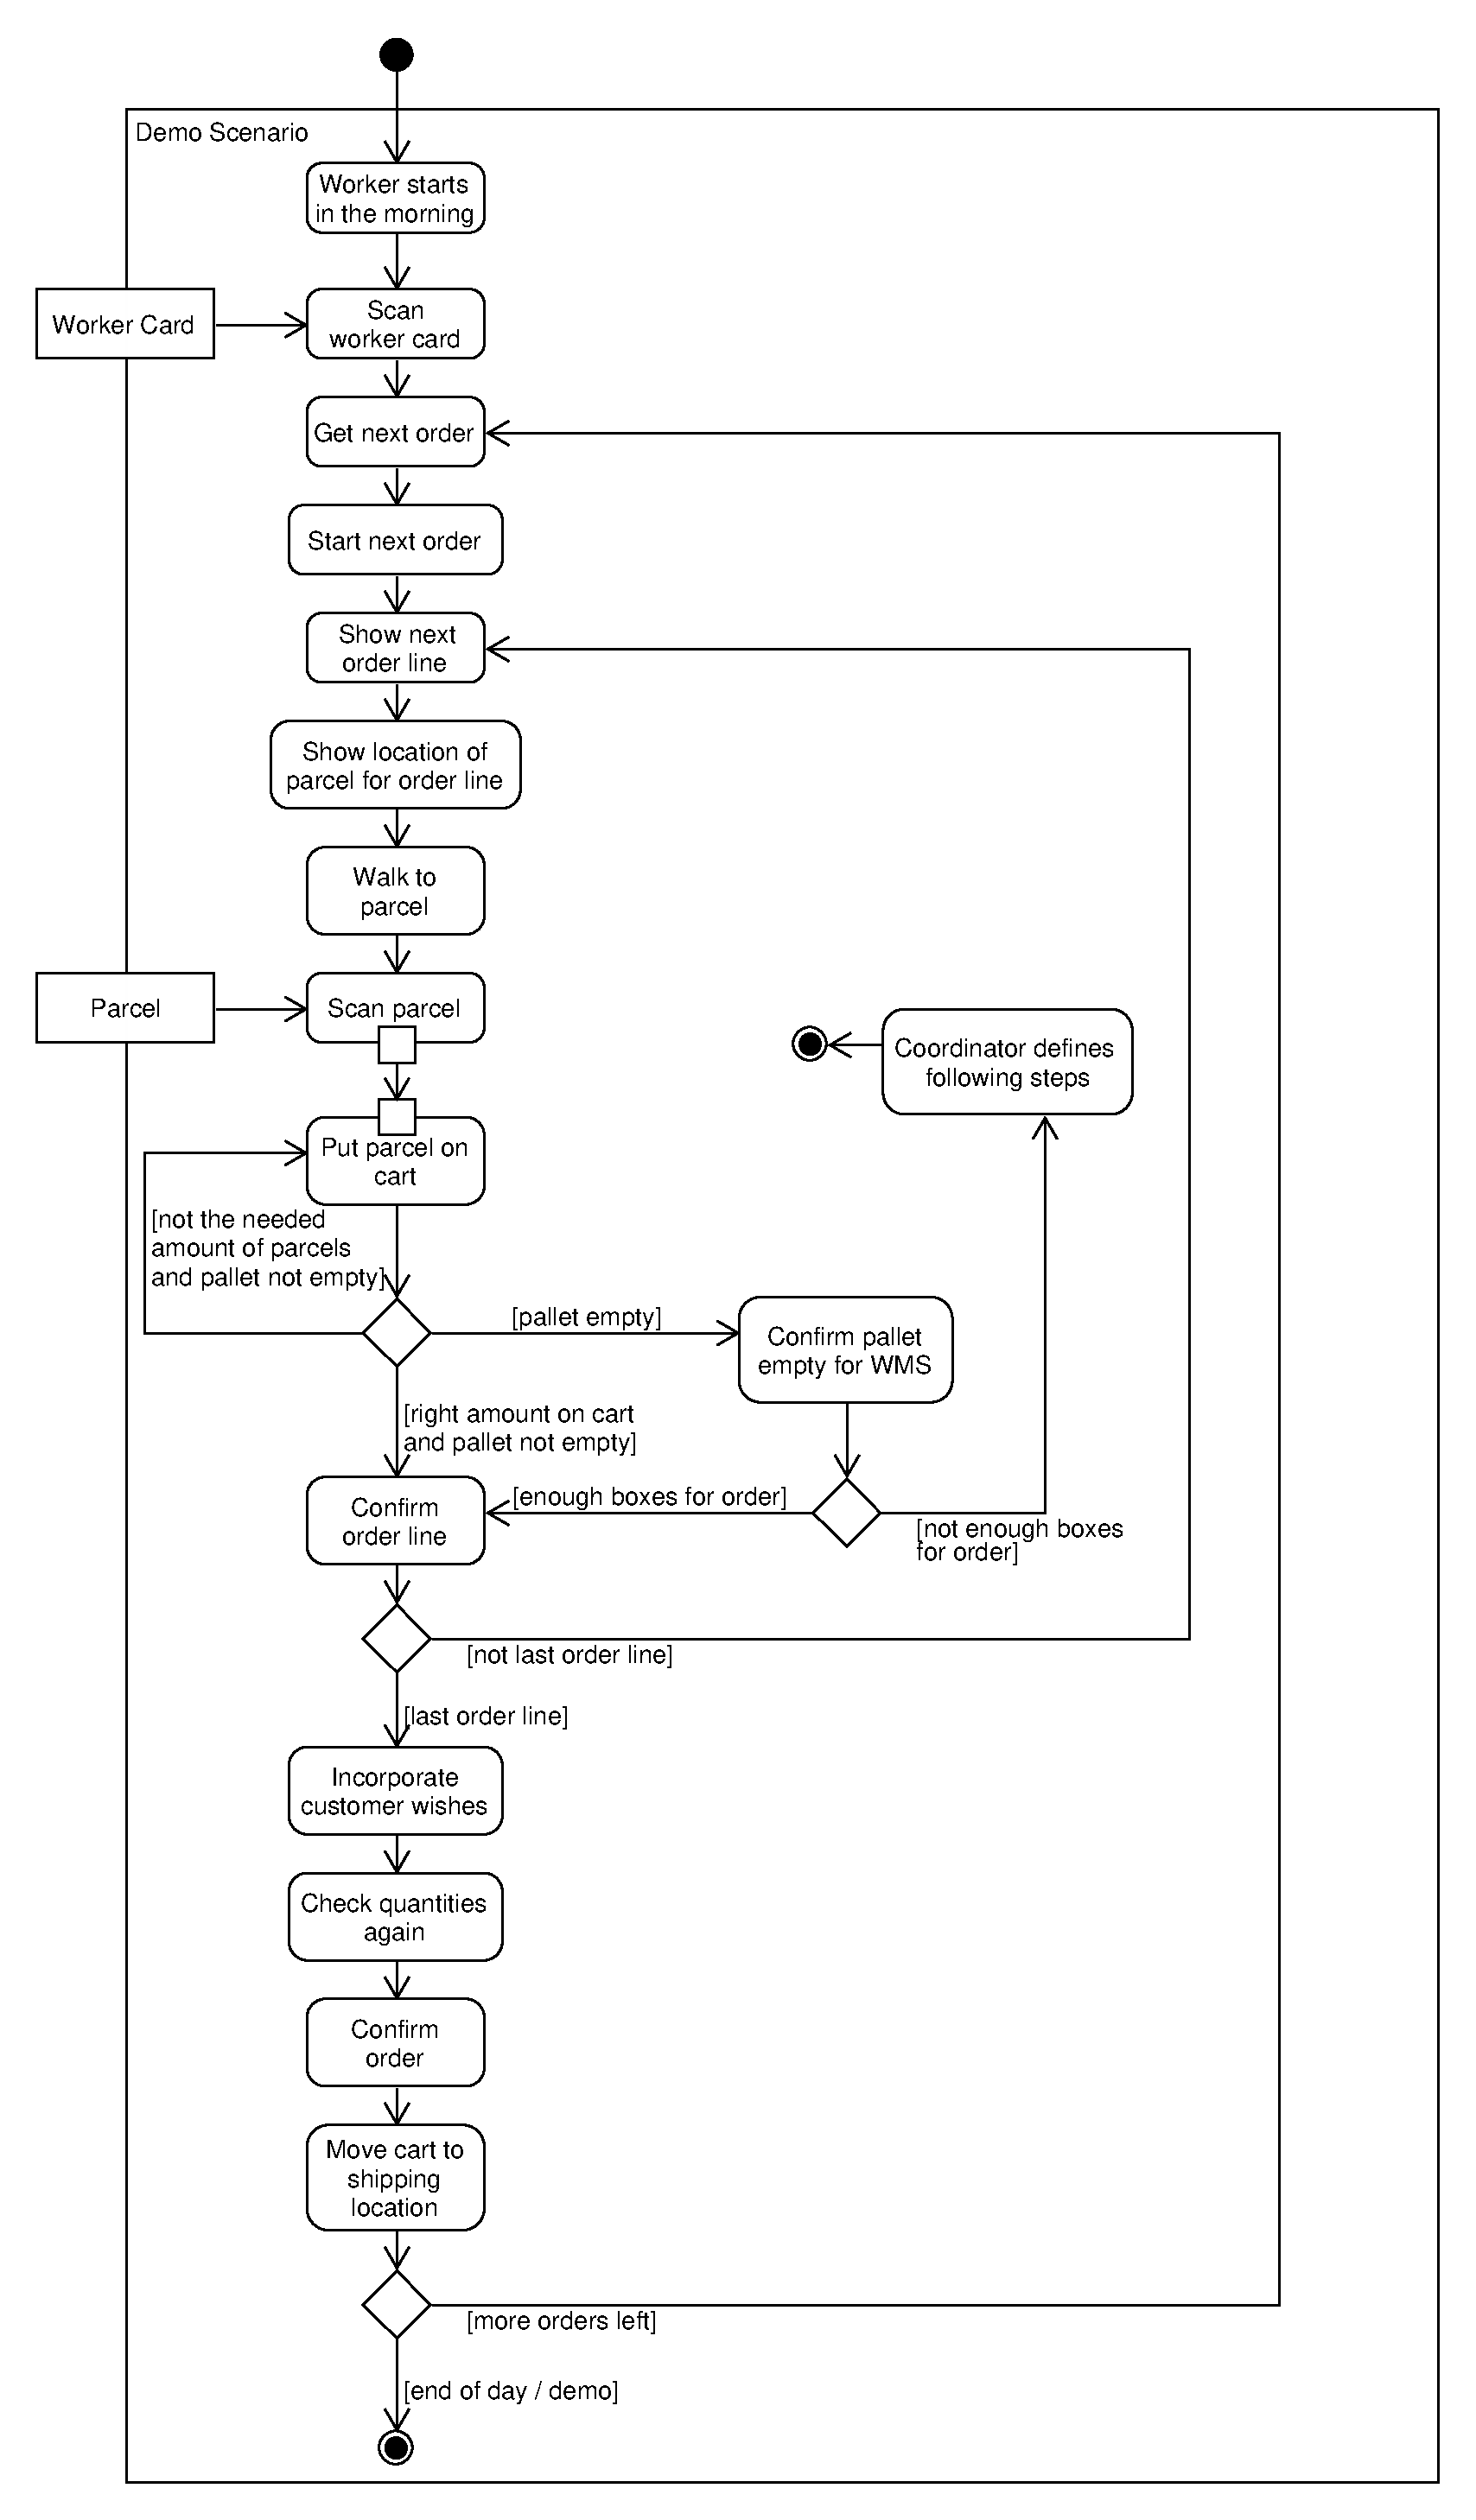
\includegraphics[height=\textheight]{images/activityDiagram_demoScenarioNoExceptions}
	\end{center}
	\caption{Activity Diagram Demo Scenario}
	\label{fig:activityDemoScenario}
\end{figure}

\clearpage

The model shows the original process in a simplified form. It also shows a complete work day and not just the process of picking a single parcel  The worker arrives in the morning and scans their worker card, this is done to log in the worker into the system and be able to get the orders that are allocated to that worker. The next thing is to get the order document, this is currently done on paper, but the intent for this is, that in the end this can be displayed on the wearable. The worker can then at first look at the order document and then continues to start working on that order. 

The order is split up into multiple order lines. An order line contains a single article, location, quantity and a number to identify the order line. The worker identifies the location and starts moving to the article location. At the article location the parcel is scanned and afterwards put on the handcart of the worker. This is repeated until the quantity listed in the order line is met. When the quantity of the order line is met, the order line is confirmed, but there are multiple things that might happen during this process:

\begin{description}
	\item[right amount on cart and pallet not empty] \hfill \\
	The process is working as explained above and the order line is confirmed without a problem.
	\item[right amount on cart and pallet empty] \hfill \\
	The pallet is confirmed empty for the \gls{wms}, but otherwise the process is working as explained above and the order line is confirmed.
	\item[too little amount of parcels on cart and pallet empty] \hfill \\
	The pallet is confirmed empty for the \gls{wms}, afterwards a coordinator is contacted to define the following steps, the process as planned is ending at this point and the steps, as defined by the coordinator are executed.
\end{description}

When the order line is successfully confirmed the next order line can be worked on, if the current order line was not the last one of the order. When the order line was the last order line the customer wishes can be incorporated. The quantities for the order will then be checked again and afterwards the order is confirmed. The handcart is then moved to the shipping location. When the order is delivered to the shipping location the next order can be started. If this is the end of the working day for the worker, the process ends.


This diagram was created for multiple reasons:

\begin{description}
	\item[Readability] \hfill \\
	The scale of the original process diagram made it hard to process. One goal was to create a more compact diagram. This was realized by designing it with the \gls{uml} 2.5 notation as specified by the \gls{omg}. \citep{manual:umlnotation}
	\item[Purpose] \hfill \\
	The original diagram had a different purpose, it was supposed to model the process of one of the pilot companies in its entirety. The purpose of the activity diagram is to model a demo case, that does not need to show every single detail of the process in the first place.
	\item[Focus point] \hfill \\
	The demo scenario focuses on the general tasks an order picking worker is doing, but is just focussing on the main points for this. The original diagram also includes the connections to the database and also includes tasks outside of the actual order picking.
\end{description}

\section{Design}
The general design for the demo facility application is based on the reference model described in chapter \ref{cha:reference}. The more concrete model for the demo facility can be seen in figure \ref{fig:ClassDiagramL1}.

\begin{figure}[t]
	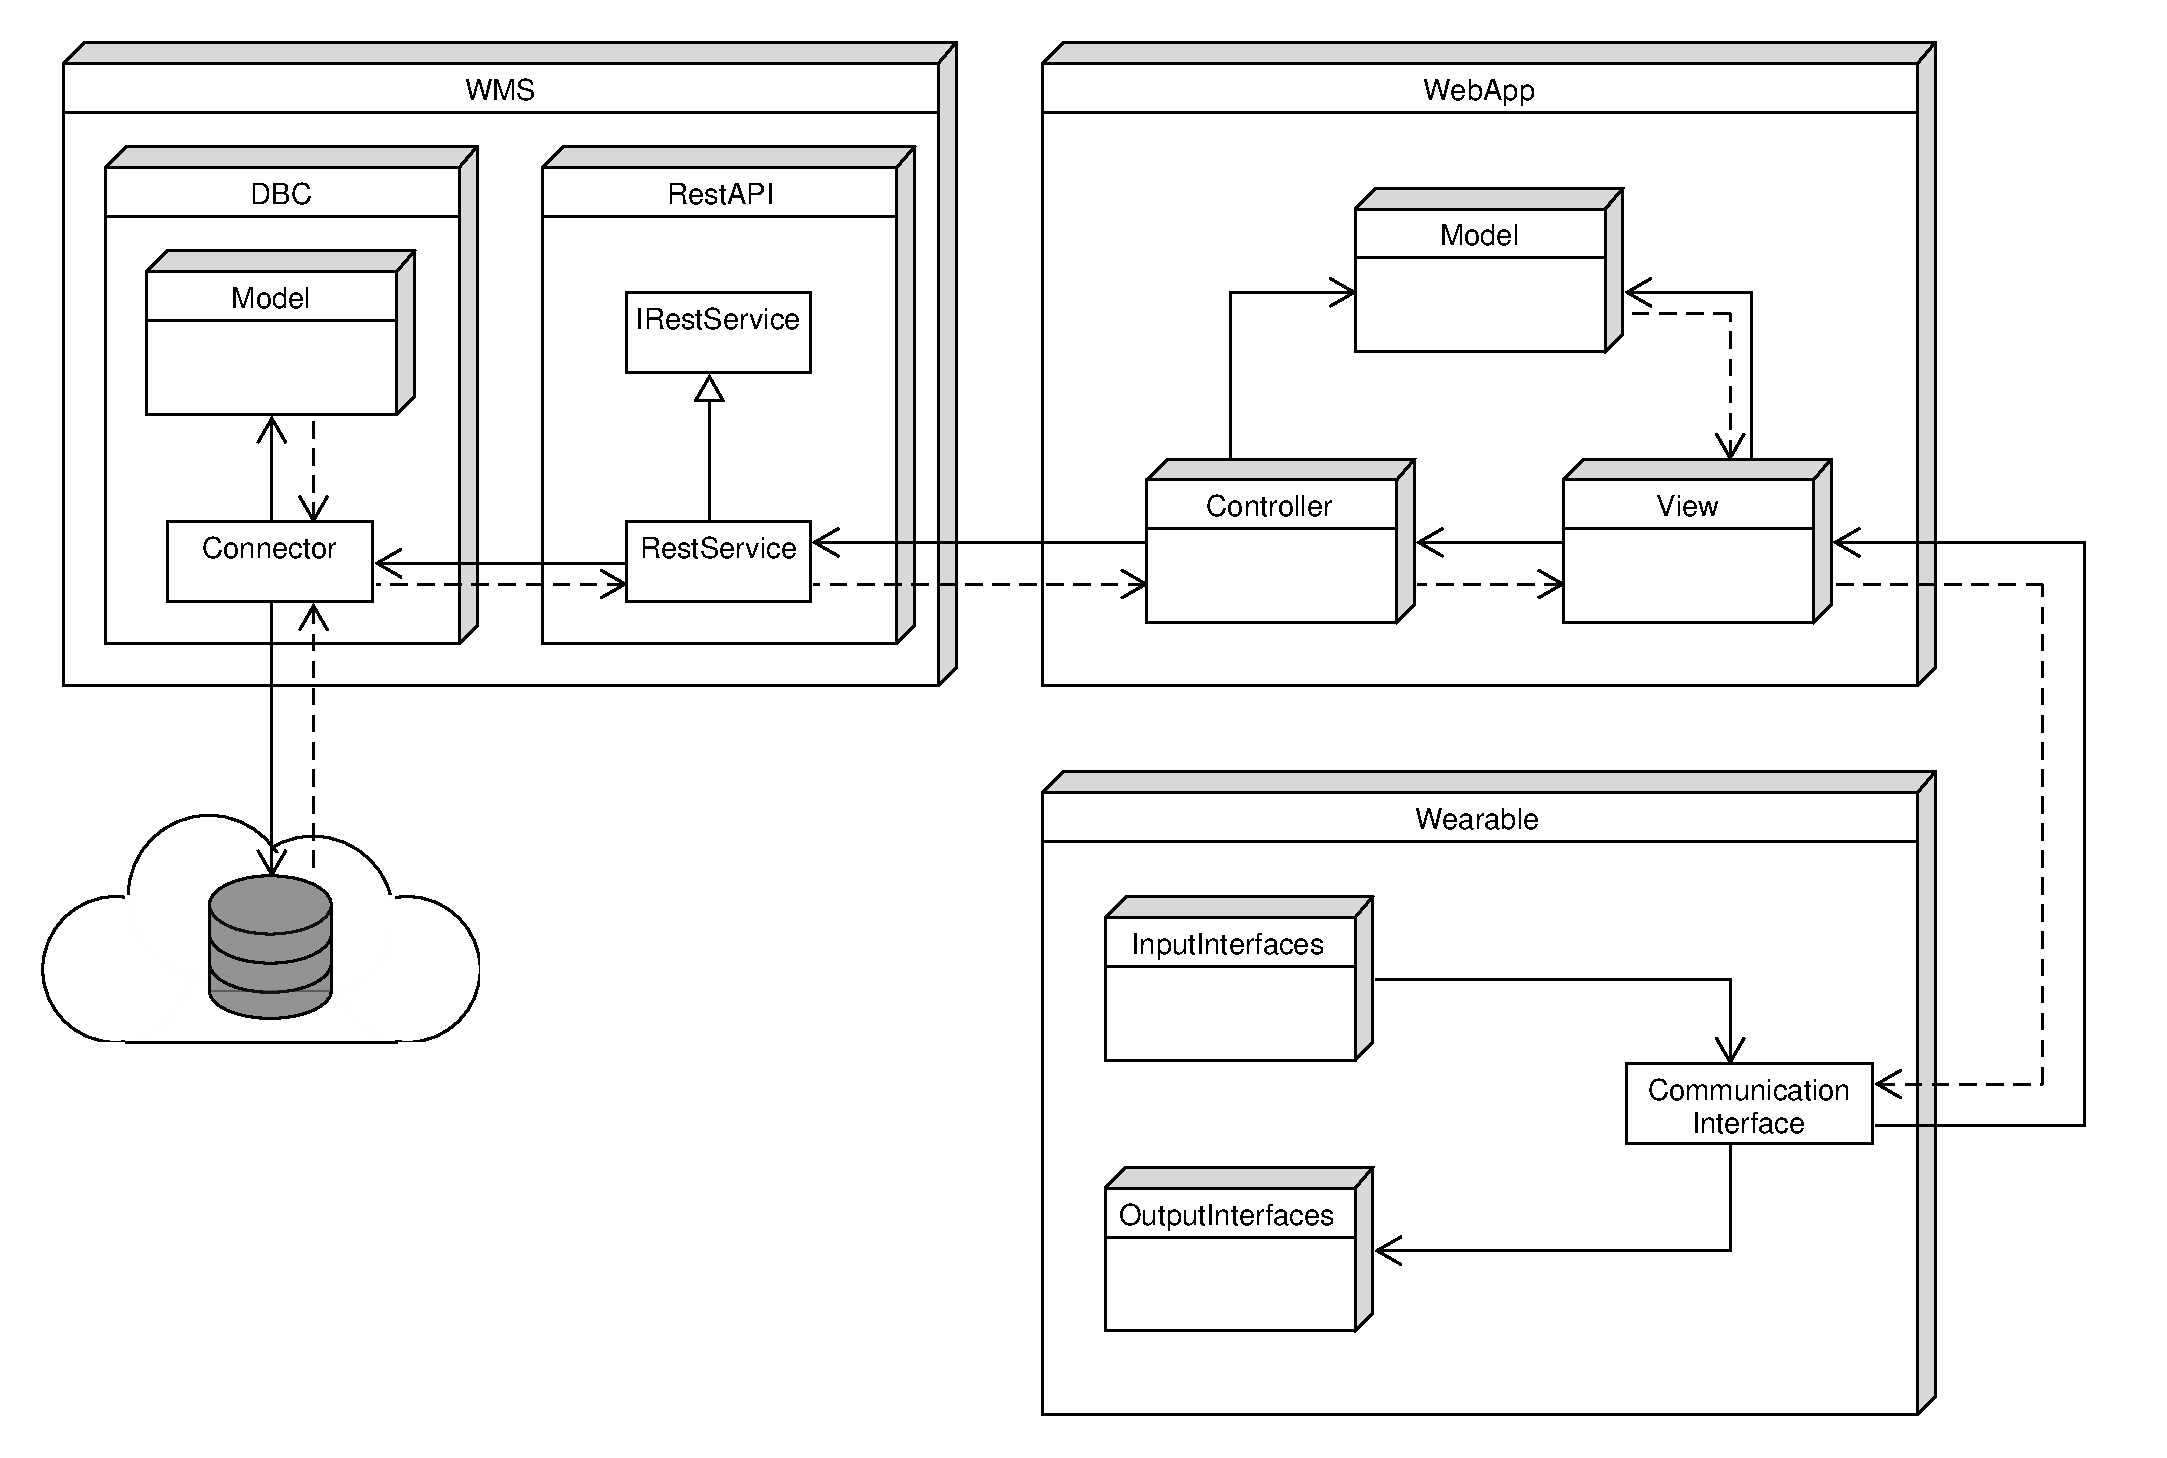
\includegraphics[width=\textwidth]{images/ClassDiagram_Level1}
	\caption{Package Diagram Demo Facility}
	\label{fig:ClassDiagramL1}
\end{figure}
The package diagram displayed is a high level view on the demo facility. The biggest difference to the reference model is the wearable, which in this case uses a thin client to connect to a web application that is doing most of the work for the wearable. The web application then in turn connects to the \gls{wms} and is replacing the communication layer that is existing in the reference model.

The normal lines represent function calls and the dashed lines represents returned information in the diagram. The following sections will go into detail for each of the displayed packages and the demo facility design will be elaborated further.


\subsection{WMS}
The \acrlong{wms} consists of two parts, the database that is going to contain the data for the demo facility and the database connector. This also defines the interface, with which to connect to the \gls{wms}.

\subsubsection{Database}

Figure \ref{fig:LogicalModelWMS} shows the relations and fields in the database. It can be seen that the database just contains a small amount of information, due to being a demo, an actual \gls{wms} would contain a lot more data. The most important item in the model is the order, as that is the key piece, where most relations lead together. An order has a number that is connecting it to one or multiple workers that are working on them. Furthermore an order consists of multiple \texttt{OrderLine}s. An \texttt{OrderLine} is describing the different lines that would appear on an order, that specify the item and the amount for an order. For a warehouse it is also important to add the pallet where to find the item and if the current line is already acknowledged or not. A pallet has a location in the warehouse and how much of that item are still available in the warehouse. The article corresponds to a name for the article number. Finally an order is ordered by a customer, a customer might have additional wishes for their orders and an address where that customer wants things delivered to.

\begin{figure}[H]
	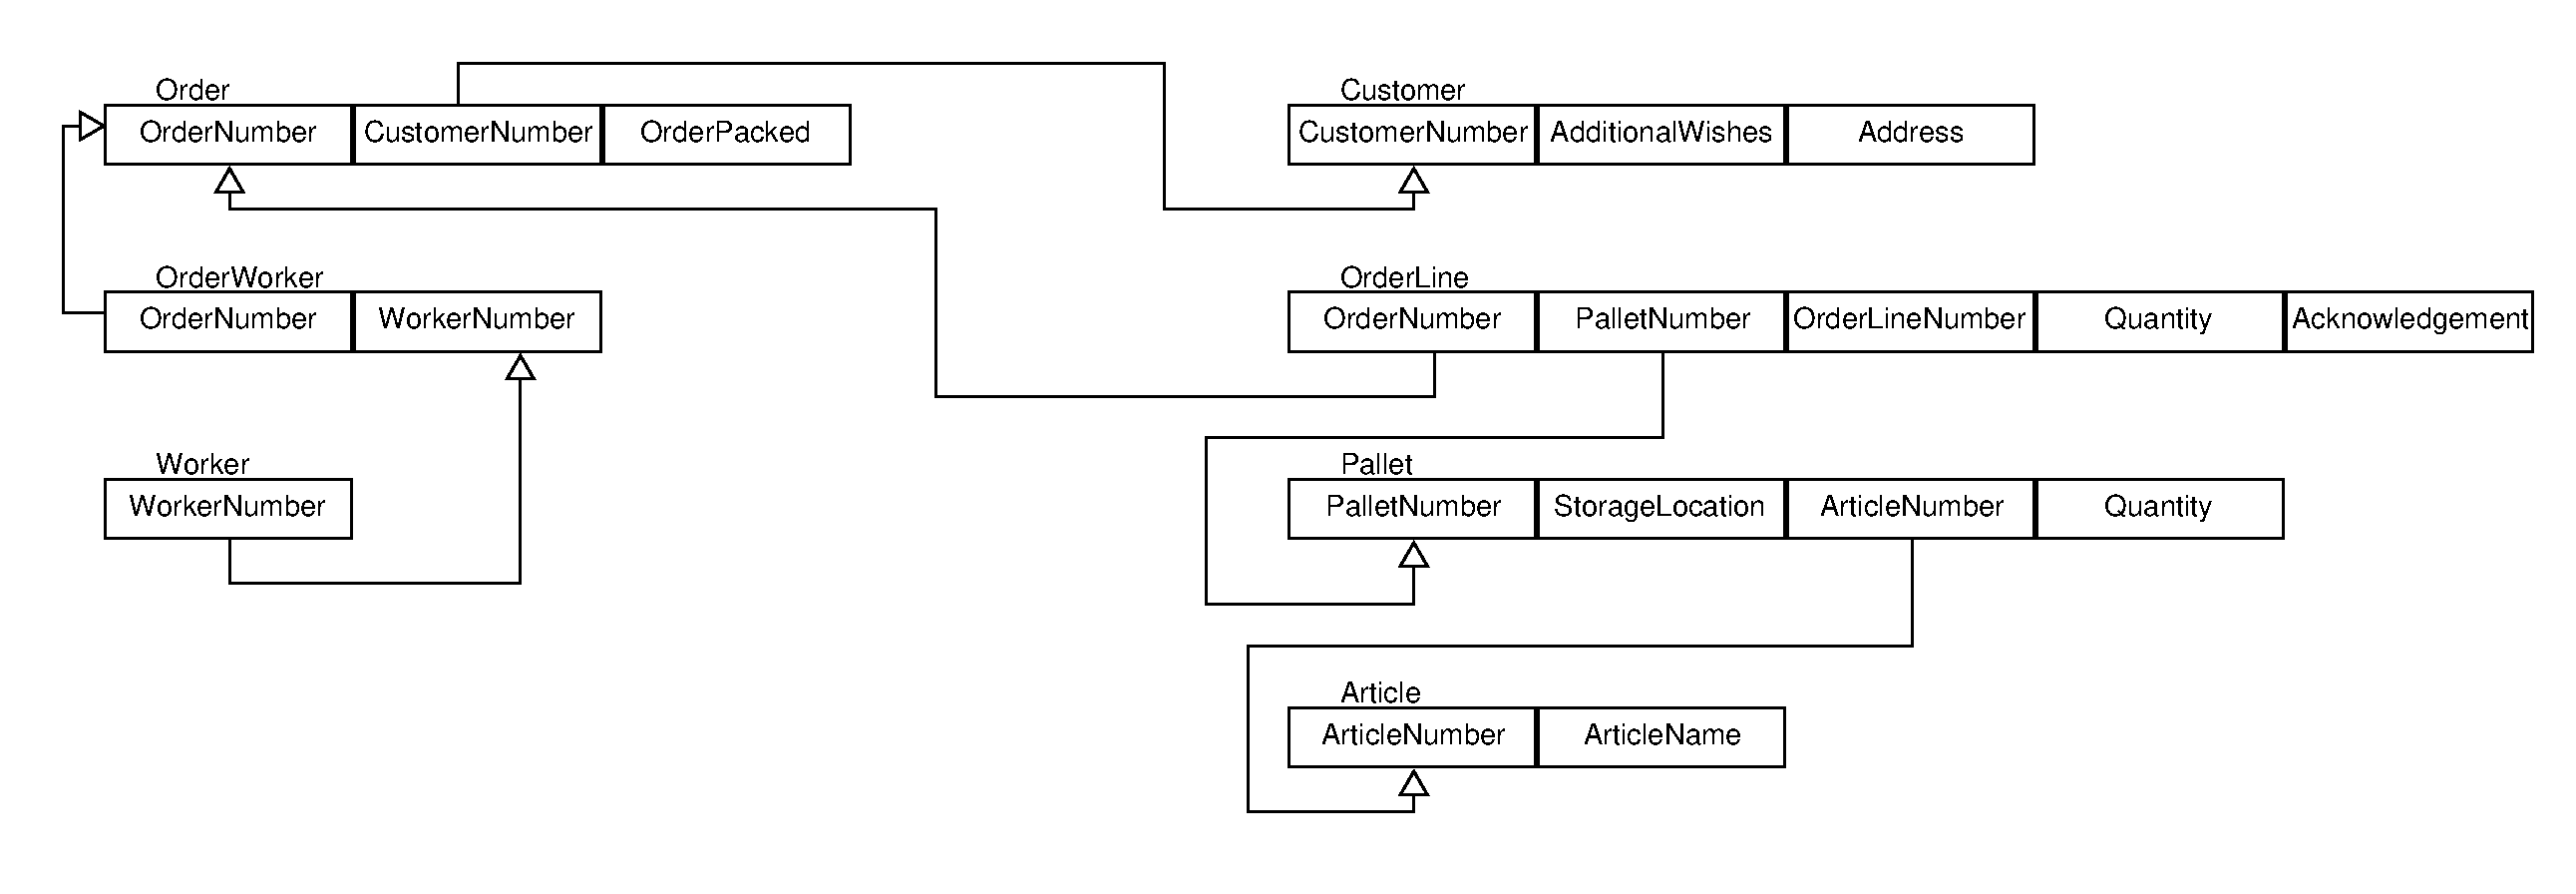
\includegraphics[width=\textwidth]{images/LogicalModel_MockWMS}
	\caption{Relational Schema Warehouse Database}
	\label{fig:LogicalModelWMS}
\end{figure}

For an actual warehouse the customers attributes would change completely, as companies might have multiple addresses, therefore that might change for every order of that customer, making it easier to add an address field to the order and not the customer.  Also a customer might want to add additional wishes just to a specific order or dependent on what might be ordered, therefore the additional wishes might also be moved to the order, but for a demo case, that is not executed at a pilot company, the model is sufficient.

\subsubsection{Interface}
The interface, that is exposed by the \gls{wms}, is a \gls{rest} interface. The options available through the \gls{rest} interface are the following:
\begin{description}
	\item[NextOrder] \hfill \\
	Returns the order with the smallest number for a specific worker.
	\item[ConfirmOrderLine] \hfill \\
	Confirms that an order line in an order has been successfully been picked.
	\item[ConfirmOrder] \hfill \\
	Confirms that a complete order has been picked.
	\item[ResetDatabse] \hfill \\
	A function that exists purely to have an existing and repeatable demo case. This resets the database to a state it was in at the beginning, before the demo was executed.
\end{description}

\subsection{Wearable}
The wearable is implemented with a \gls{thinclient}. This has multiple advantages, especially for such a demo case where potentially multiple wearables are supposed to be tested. One advantage is, because wearables tend to be less powerful devices just due to their size, the \gls{thinclient} allows to ease the load that would normally be computed on the wearable. But the bigger advantage is, that this allows to employ multiple wearables more easily. A \gls{thinclient} is implemented faster and easier than a \gls{fatclient}, therefore multiple demos for multiple wearables are more easily implemented. This allows to deploy multiple demos a lot easier. At the same time this allows a company a smoother upgrade process, meaning if they ever want to replace their existing wearables to another set of wearables, the transition could be realized a lot cheaper and faster.

Therefore apart from the usage of the input and output information to get information from the user and return information to the user only a communication interface is used to 

\subsection{Web Application}
The web application is split into multiple web pages that leads a worker through the day. The first window shown is a page, where the worker is prompted to log in by scanning their worker id. Then the next order for that worker can be started. Then order lines are displayed in more detail and can be confirmed. If every order line is confirmed the order can be confirmed and the next order can be started. The mockups for these web pages can be found in the appendix in section \ref{sec:webappmockups}.

From a technical perspective, the web application will be implemented using Java and the \gls{jsf} framework. \gls{jsf} is a part of the \gls{jee} platform and is the current standard to implement web applications with Java. Furthermore \gls{jsf} is a framework that is using the \gls{mvc} pattern to deploy web applications. 

This was chosen as the framework to implement the web application due to familiarity with the technology and it being a framework that allows rather easily to implement multiple web pages and connect that to a controller in the back end.